\documentclass{article}
\usepackage[utf8]{inputenc}

 
\usepackage{amsthm}
\usepackage{amsmath}
\usepackage{amssymb}
\usepackage{enumerate}
\usepackage{graphicx}
\usepackage{epstopdf}

%\usepackage[urw-garamond]{mathdesign}
%\usepackage[T1]{fontenc}

\newtheorem{thm}{Théorème}[section]
\newtheorem{lem}{Lemme}[section]
\theoremstyle{definition}
\newtheorem{definition}{Definition}[section]

\renewcommand*{\proofname}{Preuve}
\renewcommand{\qedsymbol}{$\blacksquare$}

\renewcommand{\baselinestretch}{1.2}
\setlength{\parskip}{5pt}
%\setlength{\topsep}{1pt}

\newcommand{\R}{\mathbb{R}}
\newcommand{\Z}{\mathbb{Z}}
\newcommand{\N}{\mathbb{N}}
\newcommand{\C}{\mathbb{C}}
\newcommand{\Q}{\mathbb{Q}}
\newcommand{\dist}{\text{dist}}
\newcommand{\Lhex}{L_{\test{hex}}}
\newcommand{\Ltri}{L_{\test{tri}}}
\newcommand{\Ghex}{\mathcal{G}_{\text{hex}} }
\newcommand{\Hex}{\mathcal{H}}
\newcommand{\hex}{\text{hex}}
\newcommand{\Gtri}{\mathcal{G}_{\text{tri}}}
\newcommand{\Tri}{\mathcal{T}}
\newcommand{\tri}{\text{tri}}
\renewcommand{\g}{\text{gauche}}
\renewcommand{\d}{\text{droite}}

\begin{document}

\section{Définitions}

Le \emph{pavage hexagonal} est le pavage du plan euclidien constitué d'hexagones réguliers. Nous nous intéresserons à son graphe simple associé, caractérisé comme $\Ghex = (\Hex, A_{\text{hex}})$, où $\Hex$ est l'ensemble des \emph{hexagones} et $A_\hex = \{(p,p') \in \Hex \times \Hex\ | \text{$p$ et $p'$ sont adjacents}\}$ est la \emph{relation d'adjacence hexagonale}. Pour tout sous-ensemble fini $U \subset \Hex$, on dit que $\Ghex[U]$ est un \emph{polyhexagone} s'il est connexe. Les \emph{polytriangles} sont définis similairement.

Soit $G = (V,E)$ un graphe simple quelconque. On dit qu'un sommet $u \in V$ est une feuille si et seulement si $\text{deg}(u) = 1$, et on écrit $n_1(G)$ le nombre de feuilles de $G$. La \emph{taille} de $G$ est le nombre de sommets de $G$, écrit $n(G)$.
La \emph{profondeur} d'un sommet $v$ dans un arbre $T$ est définie récursivement ainsi:
\[
   prof_T(v) =
   \begin{cases}
      0, \qquad & \text{si} \text{deg}_T(u) \leq 1; \\
      1 + prof_{T'}(u), & \text{sinon},
   \end{cases}
\]
où $T'$ est l'arbre obtenu en retirant toutes les feuilles de $T$.

Nous nous intéresserons alors aux polyhexagones et polytriangles acycliques, dits \emph{arborescents}. Le nombre maximal de feuilles pour un polyhexagone ou polytriangle arborescent à $n$ cellules est dénoté $\Lhex(n)$ et $\Ltri(n)$, respectivement.

\section{Démonstration}

Pour tout entier $n \geq 2$, soit la fonction $l(n)$ telle que
\begin{equation}
   \label{eq:l}
   l(n) = 
         \lfloor n/2 \rfloor + 1.
\end{equation}
Nous allons démontrer que $\Ltri(n) = \Lhex(n) = l(n)$.

\begin{lem}
   Pour tout $n \geq 2$, $\Lhex(n) \geq l(n)$ et $\Ltri(n) \geq l(n)$.
\end{lem}
\begin{proof}
   Nous allons construire une famille de polyhexagones $\{ H_n\ |\ n \geq 2\}$ dont le nombre de feuilles est donné par $l(n)$, et pour laquelle il existe une famille isomorphe de polytriangles.
   
   \begin{figure}[h!]
   \caption{La famille de polyhexagones $I_n$}
   \label{fig:In}
   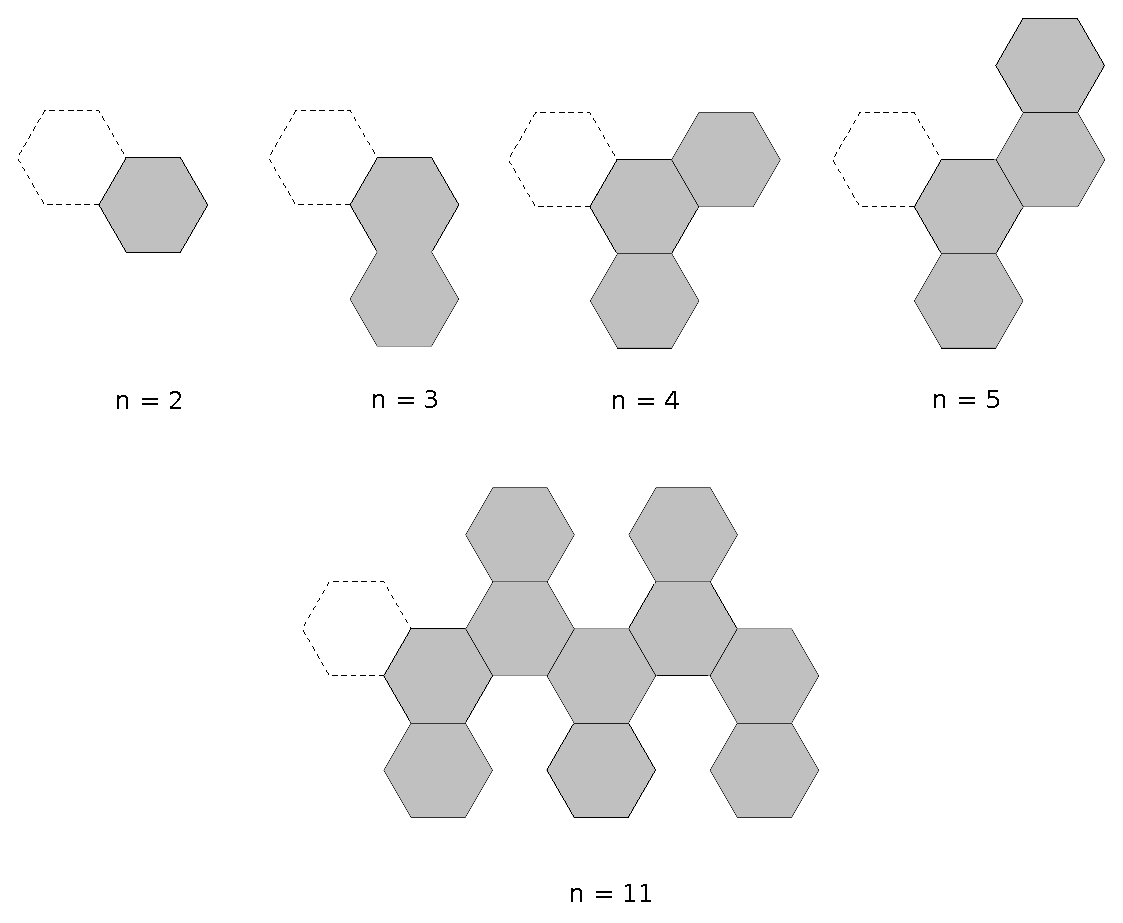
\includegraphics[width=\textwidth]{In.eps}
   \end{figure}

   Pour ce faire, nous allons commencer par définir une famille auxiliaire de polyhexagones à $n - 1$ cellules, $\{I_n | n \geq 2\}$ (figure \ref{fig:In}), à laquelle nous ajoutons un hexagone supplémentaire vers la gauche. Pour $n>5$, $I_n$ est construit en collant $\lfloor \frac{n-1}{4} \rfloor$ fois $I_5$, puis en ajoutant $I_{(n \mod 4)}$ à la droite. On remarque que $I_n$ gagne une feuille à chaque bond de 2, et que l'hexagone supplémentaire rajoute une feuille, d'où la formule en \eqref{eq:l}. 
\end{proof}

\begin{lem}
   \label{lem:hyp}
   Soit $T$ un polyhexagone ou un polytriangle arborescent de taille minimal tel que $n_1(T) > l(n(T))$ et soit $T'$ un polyhexagone ou un polytriangle arborescent tel $n(T) = n(T') + 2$. Alors
   \[
      n_1(T) > n_1(T) + 1.
   \]
\end{lem}

\begin{proof}
   Premièrement, remarquons que $l(n + 2) = l(n) + 1$. En effet,
   \begin{align*}
      l(n+2) &= \lfloor \frac{n+2}{2} \rfloor + 1 \\
             &= \lfloor n/2 + 1 \rfloor + 1 \\
             &= \lfloor n/2 \rfloor + 1 + 1 = l(n) + 1.
   \end{align*}
   Ainsi,
   \begin{align*}
      && n_1(T) &> l(n(T)), && \\
      &&      &= l(n(T') + 2), && \\
      &&       &= l(n(T')) + 1, &&  \\
      &&       &\geq n_1(T') + 1 && \text{par minimalité de $T$.}
   \end{align*}
\end{proof}

\begin{lem}
   Pour tout $n \geq 2$, $\Lhex(n) \leq l(n)$ et $\Ltri \leq l(n)$.
\end{lem}

\begin{proof}
   Supposons, en procédant par contradiction, que $T$ soit un polyhexagone ou polytriangle arborescent de taille minimale tel que $n_1(T) > l(n(T))$.

   Premièrement, remarquons que tous les sommets de $T$ de profondeur 1 sont de degré 3. En effet, si un sommet $u_1$ de profondeur 1 était de degré 2, on pourrait allors supprimer la feuille adjacente à $u_1$ et obtenir un arbre de taille plus petite sans perdre de feuilles, et $T$ ne serait alors pas minimal. De plus, dans le cas des polytriangles, un sommet ne peut avoir plus de trois voisins; et dans le cas des polyhexagones, avoir plus de 3 voisins créerait un cycle.

   Deuxièmement, $T$ ne peut pas avoir de sommet de profondeur 2. Supposons qu'un tel sommet $u_2$ existe. Alors $u_2$ doit avoir un voisin de profondeur 1, $v_1$. Nous avons vu que $v_1$ devait avoir trois voisins. Deux d'entre eux sont nécessairement des feuilles. Considérons alors l'arbre $T'$ obtenu en supprimant les deux feuilles adjacentes à $v_1$. On a que $n(T) = n(T') + 2$ mais $n_1(T) = n_1(T') + 1$, contredisant le lemme \ref{lem:hyp}.

   Puisque tous les polyhexagones ou polytriangles arborescents de taille supérieure à 4 ont au moins un sommet de profondeur 2, la preuve est complétée par vérification exhaustive des polyhexagones ou polytriangles arborescents de taille inférieure ou égale à 4.
\end{proof}

En combinant les lemmes précedant, on obtient aisément le théorème suivant.

\begin{thm}
   Pour tout $n \geq 2$, $\Lhex = \Ltri = l(n)$, et leur croissance asymptotique est donnée par $\frac{1}{2}n$. \hfill $\blacksquare$
\end{thm}
\end{document}
